 \section{Peering Module}
\label{sec:peering}

Peering module manages the configuration for all peers and maintains peering sessions for enabled peers. Every peer has its own configuration that can be changed via command line interface. 
But only enabled peer will have one and only one peering session that is established by using the peer's configuration. If the peer's configuration changes after its peering session gets established, some of the new changes will not be applied to the established peering session immediately. For instance, the changes of monitor side address and port cannot be applied to the existing peering session. This kind of changes can only take effect by closing the existing session and opening a new session.

Each peering session is a separate thread that basically maintains a BGP finite state machine such as initialize a tcp connection, exchange BGP open and keepalive messages with the peer and receives BGP update messages from
the peer. It also write all messages between BGPmon and the peer into the Peer Queue. There are 3 types of messages can be added into Peer Queue: messages from peer(BMF type 2), messages to peer(BMF type 1) and FSM state changes(BMF type 6).     
 
The details of peer configuration and peering session are discussed below. 

%In addition,  the peering module maintains statistics about each peer so that other modules such as the Periodic Module can report on the peer status.
%Once the socket has been created,  each peering thread maintains a BGP finite state machine(FSM) which has five states Idle, Connect, OpenSent, OpenConfirm and Established. Compared to the complete BGP finite state machine, the state 'Active' is not implemented in our system because the peering thread always initiates the connection actively and simply drops all the incoming connection from the peering routers for the security purpose.

\subsection{Peer Configuration}
Similar to BGP configuration in cisco IOS, we use peer group to simplify the peer configuration in BGPmon. If a number of peers share a common set of configuration, peer group can simplify configuration greatly. With a peer group that has the common set of configuration, to add a new peer one only needs to assign it to the existing peer group and specify a few fields if needed. Those specified fields will overwrite the same fields from the peer group. But all the other fields from the peer group will be inherited by the peer. 

Different from cisco IOS, every peer must be associated with a peer group in BGPmon. If one doesn't specify the peer group for a peer explicitly, this peer will be assign to the default peer group that holds the default configuration. The default peer group is created when BGPmon starts. In BGPmon, every user-created peer group is also inherited from the default peer group by default and it cannot be changed. The fields specified in the user-created peer group overwrites those from default peer group.

In detail, peering module maintains 2 arrays: one array stores all peers and another stores all peer groups. Each peer in the first array holds a reference to a peer group in the second array.  The default peer group is always created at first in the peer group array as it will be referred by any user-created peer group.  Figure \ref{fig:peerandpeergroup} shows the relationship between peers and peer gourps. In the example, there are 3 peers and 3 peer groups including the default peer group. The arrows indication the relationship between them. Peer1 has it own values for configure item A and B, so those values overwrite the values in its peer group "Group2". As a net result, PA1 and PB1 will be the final values for peer1. Peer2 belongs to default peer group directly and it doesn't have its own value for item B, so peer2 inherits the value of item B from default peer group and has PA2 and DefaultB as its final values. Similar peer 3 doesn't have its own value for item A and its peer group(Group1) doesn't have the value either, so peers inherits the value of item A from default peer group. Finally peer3 has DefaultA and PB3 as it configure values.

\begin{figure}[!htb]
\centering
\scalebox{0.4}{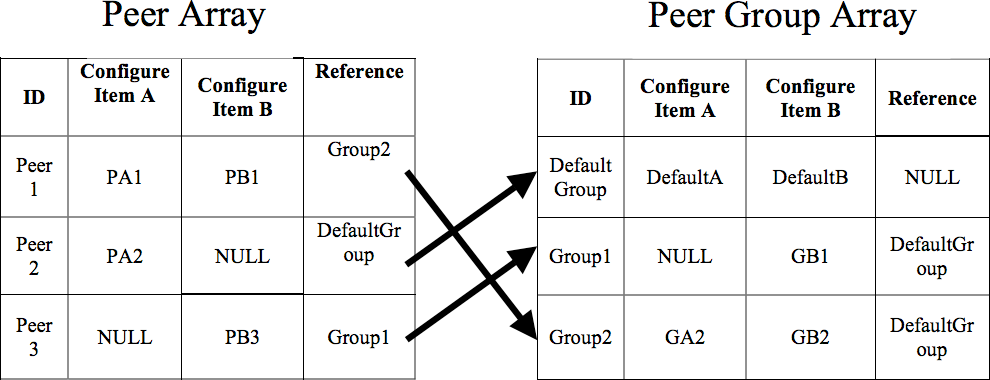
\includegraphics{figs/peerandpeergroup.pdf}}
\caption{An example of Peers and Peer Groups}
\label{fig:peerandpeergroup}
\end{figure}

From the above example, you can see the structures of peers and peer groups share the same set of configure items. In our design, peer structure and peer group structure share the same substructure "configuration" that includes all the configure items.  
Specifically peer structure consists of three parts:
\begin{itemize}
\item{\emph{Peer ID:}  It is the identifier of a peer, starting from 0. It is also the index of a peer in the array.} 

\item{\emph{Session ID:} It is  the identifier of a peering session that is associated with a peer, starting from 0. For the disabled peer, it is -1. Peering session will be discussed in the next subsection.}

\item{\emph{Configuration Substructure:} It contains all configure items needed in peer configuration.}  
\end{itemize}
And peer group structure also consists of three parts:
\begin{itemize}
\item{\emph{Peer Group ID:}  It is the identifier of a peer group, starting from 0. It is also the index of a peer group in the array.} 

\item{\emph{Peer Group Name:} It is the name of a peer group.}

\item{\emph{Configuration Substructure:} It is same as the configuration substructure in peer structure.}  
\end{itemize}
Configuration substructure includes all the configure items which are needed by peering session establishment, labeling module and periodic event handling module. Figure \ref{fig:configurationSub} shows the details of configuration substructure. All of these configure items except "routerRefreshAction" and "labelAction" are used to establish a peering session. "routerRefreshAction" is used by periodic event handling module and "labelAction" is used by labeling module.
\begin{figure*}
\centering
\scalebox{1}{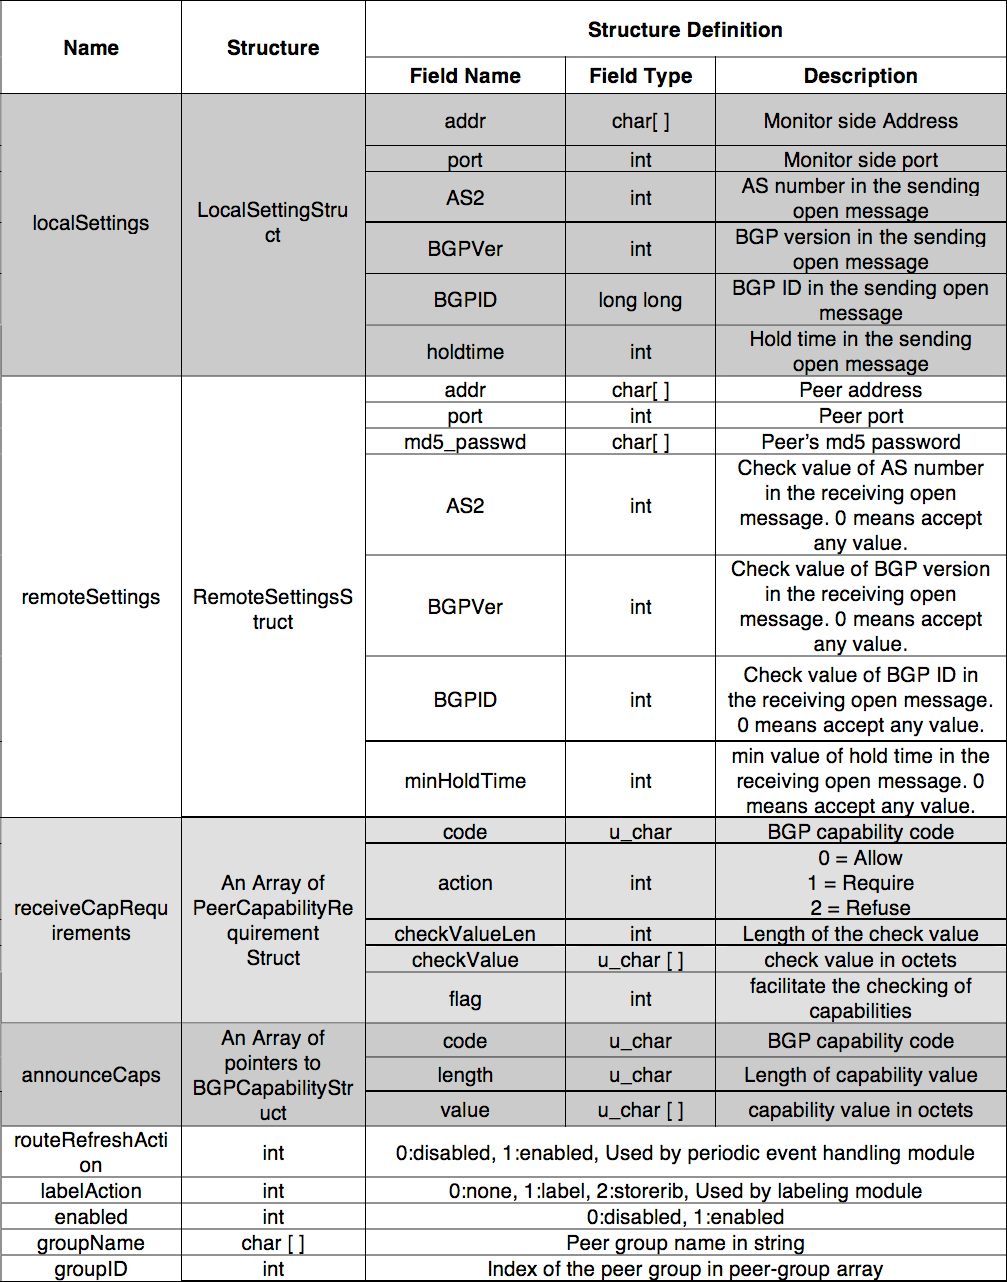
\includegraphics{figs/configurationSub.pdf}}
\caption{Configuration Substructure}
\label{fig:configurationSub}
\end{figure*}

Peering module also provides a bunch of functions to create, delete, read and write peers and peer groups.  Command line interface uses these functions to manipulate peer configuration. We have discussed the peer configuration so far. Next peering session will be discussed. 

\subsection{Peering  Session}
Peering module maintains an array that holds the data for all peering sessions and each element in this array is a "Session" structure. "Session" structure is not only used by peering module but also used by labeling module, periodic event handling module and XML module.
As we mentioned each enabled peer has its own thread and these threads create "Session" structures in the array and uses them to establish and maintain the peering sessions. In each peer's thread, a peering session gets established by using the latest configuration of that peer. When a peering session is established, all the configure items that are used to establish the session will be saved in the "Session" structure. After that, any changes in those configure items via command line interface will not take effect until the peering session resets. And the peering session could be reset in the following 2 cases.
\begin{itemize}
\item{Users reset the peering session explicitly by issuing a reset command via command line interface. This happens typically when users change some peer configuration via command line interface and want these changes to be applied immediately. } 
\item{Peering session resets by itself. For example, the underlying tcp connection failure could cause a peer session reset.  Or the peering session could be reset if the peer fails for some reason.   }  
\end{itemize}
No matter why the peering session is reset, the latest peer configuration will be used when it gets established again. 
An important design decision here is that a new "Session" structure with new session ID will be created and used by the thread every time a peering session is reset.  Note even the thread is using the new "Session" structure, the old one will still stay in the session array for a while until it is not needed. We will discuss the design philosophy behind this in the next subsection.
In the remaining part of this subsection, the detail of "Session" structure will be discussed at first and then an introduction of how to establish and maintain a peering session by using "Session" structure will be given.

\subsubsection{"Session" Structure}
\label{sec:peering:sessionstructure}
Most fields of a "Session" structure are related to the peering module and a few fields are related to other modules. The details are shown as follows:
\begin{itemize}

\item{\emph{sessionID:} is the identification of a peering session which starts from 0. It is also the index of a peering session in the array.}

\item{\emph{ConfigInUse substructure:} is same as the configuration substructure shown in Figure \ref{fig:configurationSub}.   It is basically a copy of peer configuration when peering session gets established. It will not be changed once the peering session gets established. This substructure is important if one wants to know what are the differences between the latest peer configuration and the configuration used to establish the peering session.}

\item{\emph{FSM substructure:} is a group of fields that are used to maintain the BGP Finite State Machine (FSM) such as state of FSM, socket and a couple of timers. Figure \ref{fig:FSMSub} shows the details of FSM substructure.}
\begin{figure*}
\centering
\scalebox{0.9}{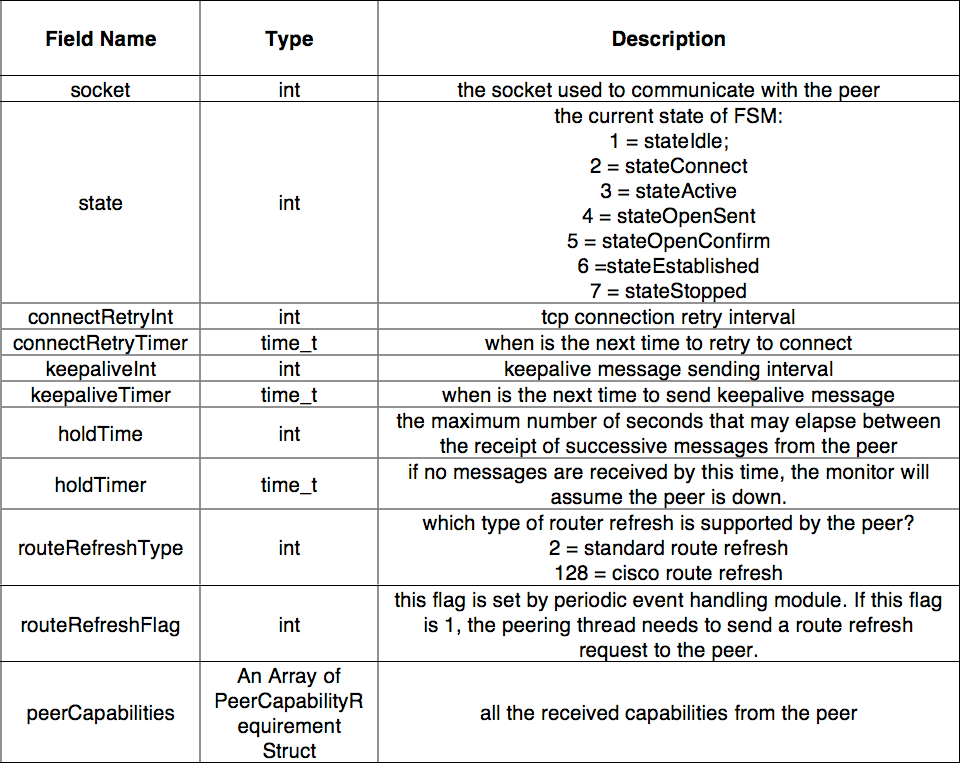
\includegraphics{figs/FSMSub.pdf}}
\caption{FSM Substructure}
\label{fig:FSMSub}
\end{figure*}

\item{\emph{Statistics substructure:} is a group of fields related to the peer's statistics such as the time of last session reset and the number of received updates. Figure \ref{fig:StatSub} shows the details of statistics substructure}
\begin{figure*}
\centering
\scalebox{0.9}{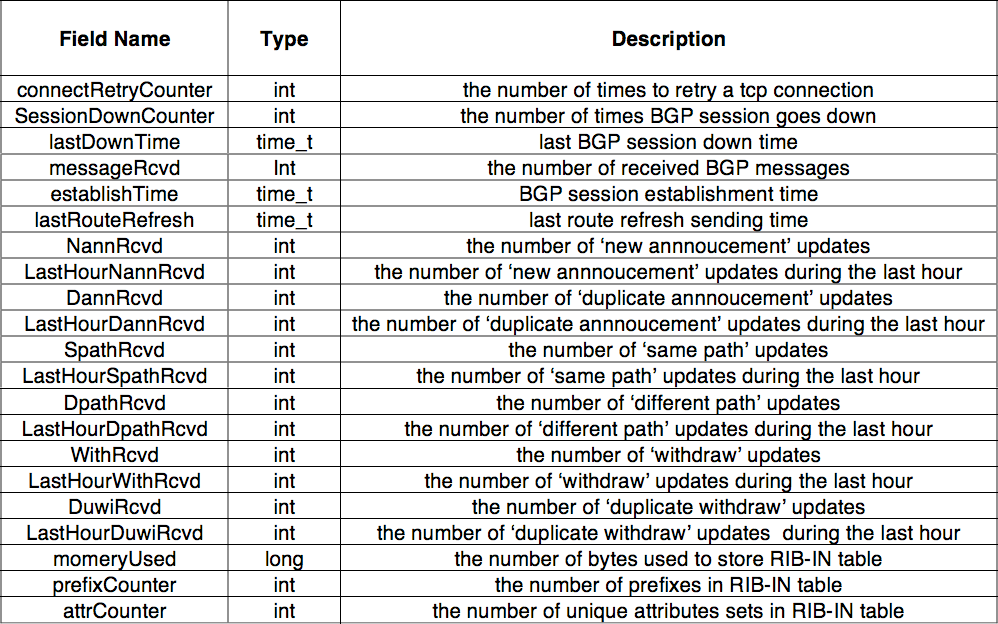
\includegraphics{figs/StatSub.pdf}}
\caption{Statistics Substructure}
\label{fig:StatSub}
\end{figure*}

\item{\emph{peerQueueWriter:} is used to write the messages exchanged between BGPmon and the peer into the queue. }

\item{\emph{sessionStringOutgoing:} is a XML string generated by peering module. It is used by XML module as the common XML header of all outgoing messages. It consists of 2 triples: Source triple and Destination triple.
Source triple contains monitor side address port and AS number.  Destination triple contains peer's address, port and AS number.   }

\item{\emph{sessionStringIncoming:} is similar to sessionStringOutgoing. It is a common XML header for all incoming messages. In this XML string, source triple contains peer address port and AS number.  Destination triple contains monitor side address, port and AS number. }

\item{\emph{PrefixTable Substructure and AttrTable Substructure:} are used to maintain a RIB table. They are initialized by peering module and populated by labeling module. The detail of them will be discussed in Section \ref{sec:labeling}. }

\item{\emph{reconnectFlag:} is used to reset a peering session and set by command line interface. This flag is typically set when a user wants the changes of peer configuration to be applied. }

\item{\emph{lastAction:} is a timestamp that indicates when the last action of a peering session is. It is used to check if a peering session is running correctly. }

\end{itemize}

\subsubsection{Establish and Maintain Peering Sessions}

To establish a BGP peering session, the first step in peer's thread is to create a socket and bind it to the monitor side address and a port specified in "localSettings" of the peer configuration( See Figure \ref{fig:configurationSub}). 
Secondly, the thread needs to initiate a tcp connection to the peer actively. Similarly, the peer's address and port are specified in "remoteSettings" of the peer configuration. Note in our design the thread always initiates the connection actively and simply drops all the incoming connection from the peer for the security purpose.

Once the tcp connection is established, the thread will exchange the BGP open message with the peer. As shown in  Figure \ref{fig:configurationSub}, all the parameters(BGP version, BGP ID, AS number and holdtime) needed to create a BGP open message can be found in "localSettings" of configuration substructure. Also all announcing capabilities included in the open message can be found in "announceCaps" of configuration substructure.
Then the thread sends the created open message via the established tcp connection and waits for the incoming open message from the peer. 

Upon receiving the open message, the thread will do the following two checks.
\begin{itemize}
\item{ Check the version, AS number, Identifier and holdtime in the received open message against the expected values specified in "remoteSetting" of configuration substructure( See Figure \ref{fig:configurationSub}). }
\item{ Check the capabilities in the received open message against the capability requirements specified in "receiveCapRequirements" of the configuration substructure(Figure \ref{fig:configurationSub}). For each capability $A$ in capability requirements, there are three possible actions:  }
\begin{itemize}
\item{ \emph{Allow:} nothing needs to be done.}
\item{ \emph{Require:} check if the received capabilities contain $A$ and the value of the received capability is same as the check value is configured. If no, check fails.}
\item{ \emph{Refuse:} check if the received capabilities contain $A$ and the value of the received capability is same as the check value is configured. If yes, check fails. }
\end{itemize}
\end{itemize}
If any of these checks fails, the thread will send a notification message to the peer and close the connection.
If all the checks pass, the thread will send a keepalive message to the peer and wait for another keepalive message from the peer. Once this keepalive message is received, the BGP peering session is successfully established. 

After the peering session gets established, the thread will periodically sent out keepalive messages if holdtime is not zero and route refresh requests if configured.

Each thread also writes two types of messages into the peer queue:
\begin{itemize}
\item{BGP Message: The BGP messages exchanged with the peer are written into the peer queue. Note no 'Update' messages will be sent from BGPmon. }
\item{FSM Message: The state changes of BGP finite state machine are written into the peer queue such as from 'Idle' to 'Connect', from 'OpenConfirm' to 'Established' and so on.}
\end{itemize}
These types of messages are converted into BGPmon internal format before being written into peer queue. After conversion, the session ID in the message indicates it belongs to which peering session.

In our design, periodic event handling module centralized manages and schedules the route refresh for all the peers. Instead of sending route refresh requests by itself, periodic event handling module notifies the peering module to send route refresh requests when needed. And the field 'routeRefreshFlag' in FMS substructure(Figure \ref{fig:FSMSub}) is used to notify peering module. 

\subsection{Design Philosophy}
In the design of peering module, one important issue is how to handle changes in a peer's configuration when the peer already has a existing peering session. Most of configuration changes will only take effect by resetting the existing peering session such as changes in monitor address, port or AS number. But it is not practical to reset a peering session every time such a change happens. Probably one might want to reset the peering session after a series of changes is done. So we decided to let the user make the decision about when to reset the peering session. User can reset the peering session by issuing a command via command line interface. 

As a result of letting user make the decision when to make configuration changes take effect, it is necessary to provide the user with the difference between the latest peer configuration and the configuration used to establish the existing peering session.
This explains why we need a "ConfigInUse" substructure in a "Session" structure. The "ConfigInUse" substructure is copied from peer configuration when peering session is established and will not be changed after that.
By comparing the "ConfigInUse" of a peering session and the latest peer configuration, the user will know all the changes of a peer configuration since its peering session was established. 

Another important design issue is that a new "Session" structure with new session ID will be created and used by the thread every time a peering session is reset. The reason is related to the BGPmon architecture and the format of BMF message.
As we discussed, modules of BGPmon are connected by queues and every message in peer queue and label queue has a session ID field. 
The session ID will be used as the key to retrieve the information needed to process the BMF messages by other modules such as labeling module and XML module.
For example, XML module needs the session ID to get the XML common header("sessionStringOutgoing" and "sessionStringOutgoing" in a "Session" Structure) in order to convert a BMF message to a XML string.
In BGPmon it is possible that some BMF messages associated with old peering session are buffered in the queue after a peering session gets reset . 
In this case if the peer's thread doesn't create a new "Session" structure and simply uses the same "Session" structure, XML module will wrongly convert the BMF messages associated with old peering session by using the XML common header of new peering session.
In order to avoid this,  the peer's thread needs to create a new "Session" structure and keep the old "Session" structure when a peering session is reset. After peering session reset, the peer's thread will use the new "Session" structure and tag the new BMF messages with new session ID.
The old "Session" structure will finally be deleted after all the BMF message associated with the old peering session are processed. 
%\subsection{Data Structure}
%The single key data structure of peering module is called session. Each peering thread is attached with a session structure. The session structure consists of five parts:
%\begin{itemize}

%\item{\emph{sessionID:} is 16 bit session identification. It is started from 1 and each peering thread is associated with a unique SessionID.}

%\item{\emph{Configuration substructure:} includes all the configurations of a peer which are needed to establish the BGP session such as peer's address and AS number. It is created by configuration module. The Configuration Module will write this section and the Peering Module will only read it.}

%\item{\emph{FSM substructure:} is a set of fields which are related the BGP Finite State Machine (FSM) used to maintain the BGP session.   The Peer Module will write and read this section.   Other modules may read this section to learn the status of a peer.}

%\item{\emph{Statistics substructure:} is a group of fields related to the peer's statistics such as the time of last session reset and the number of received updates.    The Peer Module will write and read this section.   Other modules may read this section to learn statistics about this peer.}

%\item{\emph{peerQueueWriter:} It is used to write the messages received from peers to the peer queue. }

%Figure \ref{fig:sessionStruct} shows the session structure.
%%\begin{figure*}
%%\centering
%%\caption{BGPmon Internal Message Types}
%%\label{tab:sessionStruct}
%%\end{figure*}

%%\begin{figure}[!htb]
%\begin{figure}[!htb]
%\scalebox{0.56}{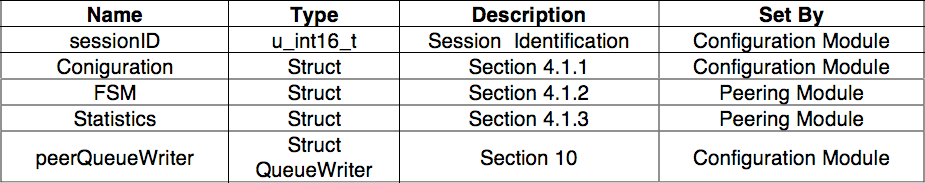
\includegraphics{figs/sessionStruct.pdf}}
%\caption{Session Structure}
%\label{fig:sessionStruct}
%\end{figure}

%%\begin{figure*}
%%\centering
%%\begin{tabular}{| l | l | l |}
%%\hline
%%sessionID & $u_int16_t $ & Session  Identification & Configuration Module\\
%%\hline
%%configuration & struct & Section 4.1.1 & Configuration Module\\
%%\hline
%%FSM & struct & Section 4.1.2 & Peering Module\\
%%\hline
%%statistics & struct & Section 4.1.3 & Peering Module\\
%%\hline
%%\end{tabular}
%%\caption{Session Structure}
%%\label{tab:sessionStruc}
%%\end{figure*}
%\end{itemize}

%\subsubsection{Configuration  SubStructure}
%Configuration SubStructure consists of six parts. 
%\begin{itemize}
%\item{\emph{BGP Open Message:}  It is the BGP open message sent to the peer in order to establish the BGP session.} 

%\item{\emph{Monitor Settings:} It contains a protocol independent address structure which is used to open the socket and a hold time used to negotiate the final hold time with the peer. }

%\item{\emph{Router Settings:} First it contains a protocol independent address structure and optional MD5 password which are used to connect to the peer. Secondly it contains the expected AS number, BGP version, BGP Identifier and minimal hold time. The received open message from the peer is checked against these expected values. }

%\item{\emph{Capability Requirements:} It contains a array of capability requirements based on the configuration. The received capabilities from the peer are checked against these capability requirements. }

%\item{\emph{Desired Configuration:} It is used to signal the peering module the changes in configuration. It will be incremented by one every time the configuration is changed by configuration module. }

%\item{\emph{Enabled:} It is used to signal the current configured peer status(pause, normal or close). It is set by configuration module.   }

%\end{itemize}
%Figure \ref{fig:configurationSub} shows the details of configuration substructure. 
%\begin{figure*}
%\centering
%\scalebox{1}{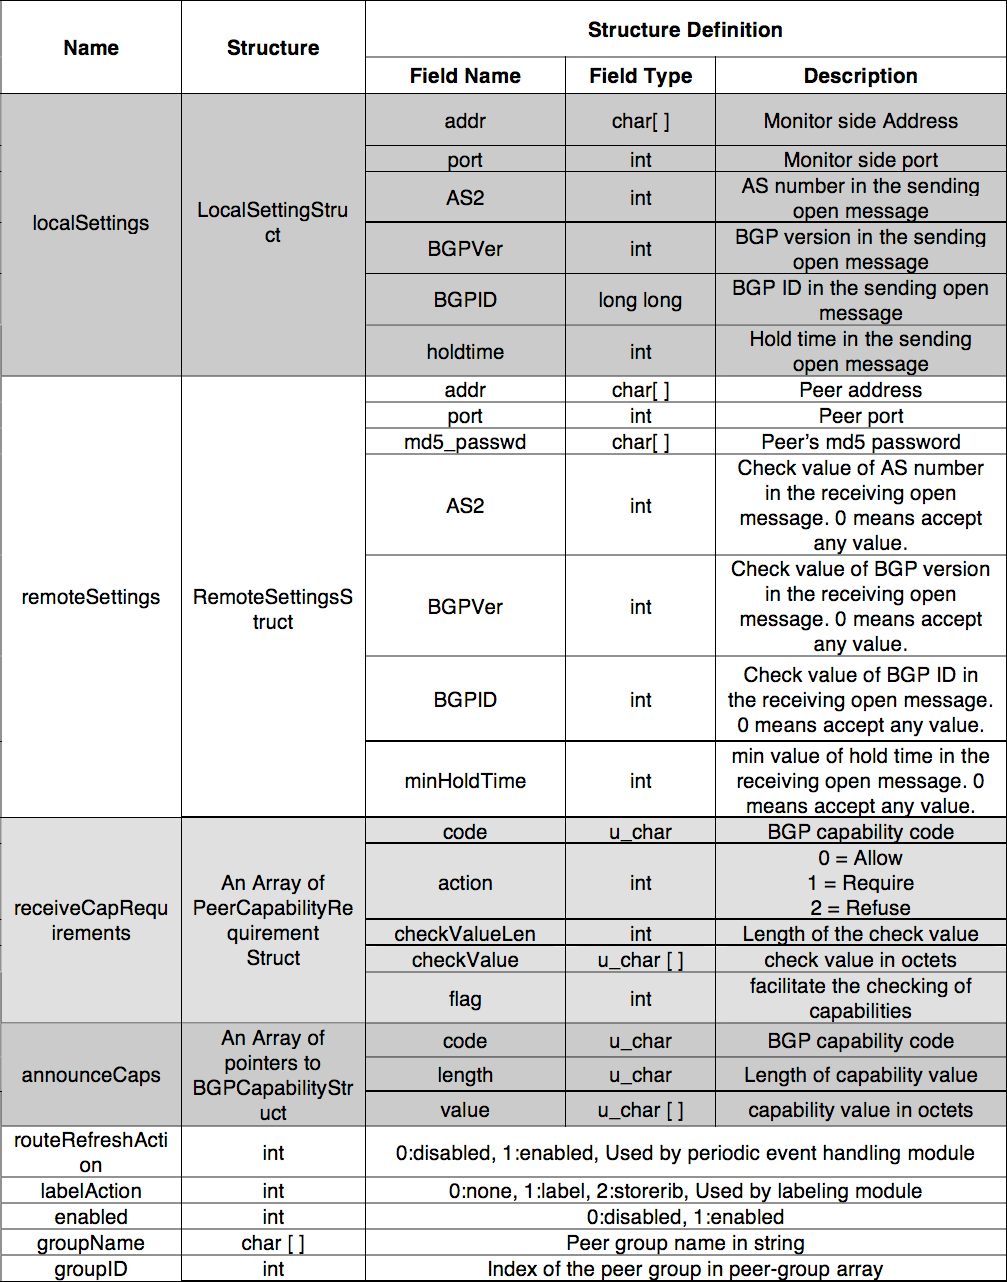
\includegraphics{figs/configurationSub.pdf}}
%\caption{Configuration Substructure}
%\label{fig:configurationSub}
%\end{figure*}

%\subsubsection{FSM SubStructure}
%FSM substructure contains all the information needed to maintain a BGP session.  It consists of a socket, the current state of FSM, and several timers.
%Figure \ref{fig:FSMSub} shows the details of FSM substructure.
%\begin{figure*}
%\centering
%\scalebox{1}{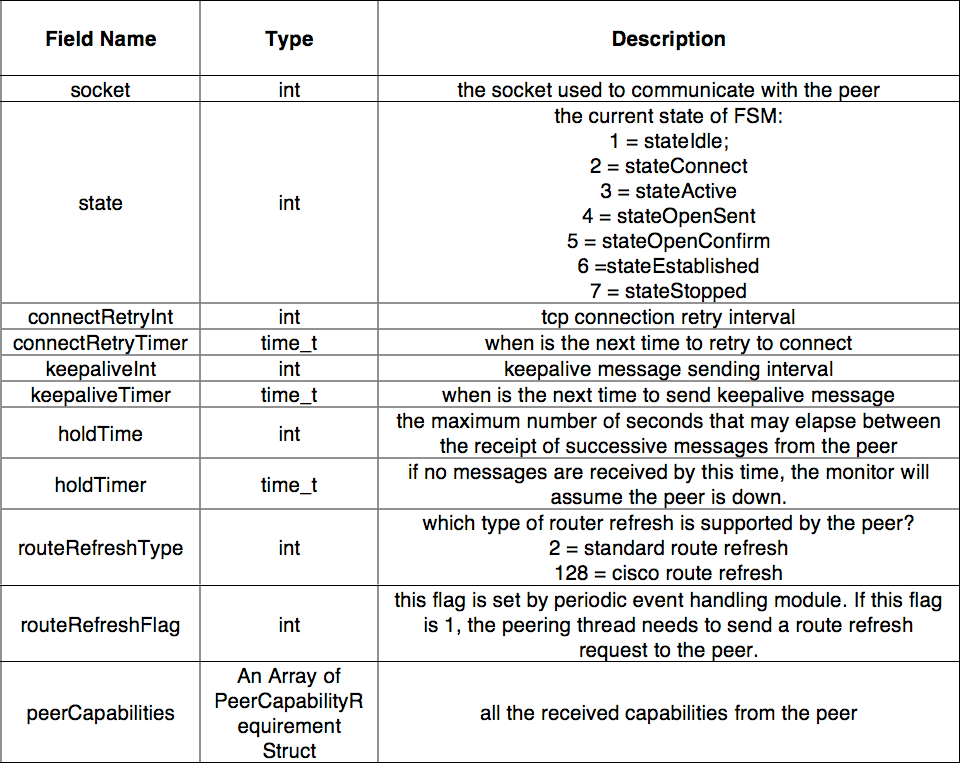
\includegraphics{figs/FSMSub.pdf}}
%\caption{FSM Substructure}
%\label{fig:FSMSub}
%\end{figure*}

%\subsubsection{Statistics SubStructure}
%Statistics substructure contains the peer's statistical information. 
%Figure \ref{fig:StatSub} shows the details of statistics substructure.
%\begin{figure*}
%\centering
%\scalebox{1}{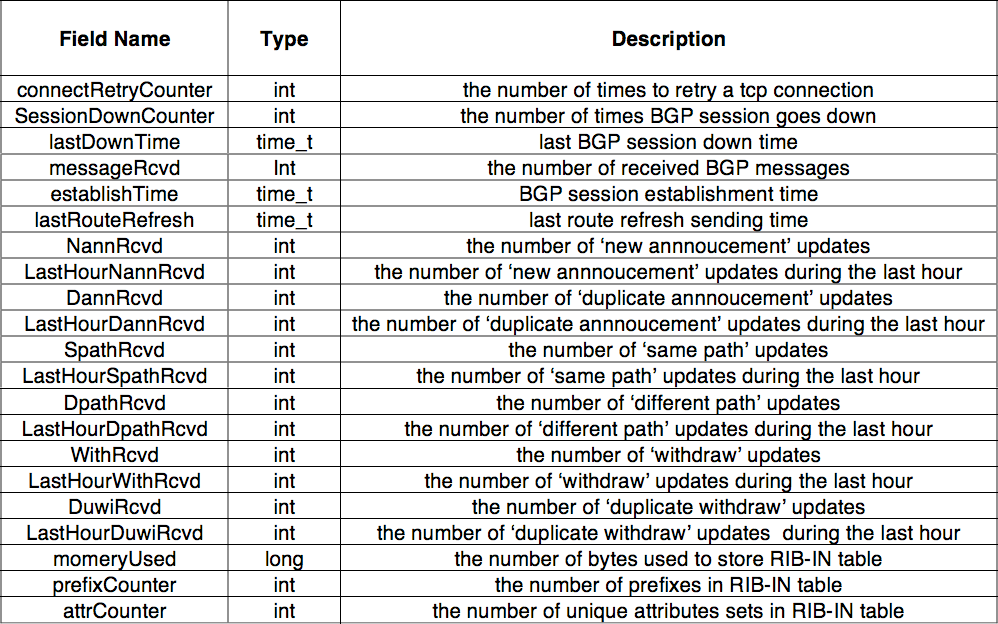
\includegraphics{figs/StatSub.pdf}}
%\caption{Statistics Substructure}
%\label{fig:StatSub}
%\end{figure*}

%\subsection{Opening and Maintaining Peering Sessions}

%% opening the socket....     note config has set address.    do not care if this is IPv4 or Ipv6 or other.
%The first step of peering thread is to create a socket and bind it to a interface and a port if configured. According to Figure \ref{fig:configurationSub}, configuration module has created monitor's protocol independent address structure.  This structure contains all the information needed to create sockets and bind sockets such as address family, socket type, address and port. So the peering thread can simply create and bind a socket with this protocol independent address structure without knowing its content such as its address family(IPv4 or IPv6) and the port number. 

%Secondly, the peering thread needs to establish the tcp connection with the router actively. Similarly, configuration module has created router's protocol independent address structure. The peering thread can establish the tcp connection by using the created socket and the router's protocol independent address structure.
%Note in our design the peering thread always initiates the connection actively and simply drops all the incoming connection from the router for the security purpose.

%Once the tcp connection is established, the peering thread will exchange the BGP open message with the peer. As we mentioned before, configuration module has created the open message and included all desired capabilities(Figure \ref{fig:configurationSub}). The peering thread just sends the created open message via the established tcp connection and waits for the incoming open message from the peer. Upon receiving the open message, the peering thread will do the following two checks.
%\begin{itemize}
%\item{ Check the version, AS number, Identifier and holdtime in the received open message against the expected values of them in the configuration substructure(Figure \ref{fig:configurationSub}). }
%\item{ Check the capabilities in the received open message against the capability requirements in the configuration substructure(Figure \ref{fig:configurationSub}). For each capability $A$ in capability requirements, there are three possible actions:  }
%\begin{itemize}
%\item{ \emph{Allow:} nothing needs to be checked.}
%\item{ \emph{Require:} check if the received capabilities contain $A$ and the value of the received capability is same as the check value is configured. If no, check fails.}
%\item{ \emph{Refuse:} check if the received capabilities contain $A$ and the value of the received capability is same as the check value is configured. If yes, check fails. }
%\end{itemize}
%\end{itemize}
%If any of these checks fails, the peering thread will send a notification message to the peer and close the connection.
%If all the checks pass, the peering thread will send a keepalive message to the peer and wait for another keepalive message from the peer. Once this keepalive message is received, the BGP session is successfully established. 

%After the BGP session gets established, the peering thread will periodically sent out keepalive messages if holdtime is not zero and route refresh requests if the peer supports it.
%   

%% sending the open message....   note config has set open message and included all desired capabilities.
%% checking the capabilities....     how does it do this?   what notifies are sent?
%%Figure \ref{fig:capstruct} show the capabilities structure used by the peering module.
%%maintaining the connection....    sending and receiving keepalives.     what if hold time is zero?   what notifies might be sent?

%Each peering thread also writes two types of messages into the peer queue:
%\begin{itemize}
%\item{BGP Message: The BGP messages sent or received by the peering threads are written into the peer queue. Note no 'Update' messages are sent from the peering thread to peering router. }
%\item{FSM Message: The state changes of BGP finite state machine made by the peering thread are written into the peer queue such as from 'Idle' to 'Connect', from 'OpenConfirm' to 'Established' and so on.}
%%\item{Peer Status Message: The states of the peer are written into the queue. The states of peer can be very simple such as the peer's address and AS number.  It also can be complex such as the BGP capabilities received from the peer. }
%\end{itemize}
%These types of messages are converted into BGPmon internal format by peering threads before being written into peer queue.

%%\subsection{Maintaining Statistics}
%% what do we maintain?     last action time,  bytes recvd, bytes sent, ??

%\subsection{Route Refresh}
%% how do we request this?
%Periodic event handling module centralized manages and schedules the route refresh for all the peers. Instead of sending route refresh requests by itself, periodic event handling module notifies the peering threads to send route refresh requests when needed. And a field 'routeRefreshFlag' in FMS substructure(Figure \ref{fig:FSMSub}) is set to notify peering thread by periodic event handling module.  Each peering thread reads this flag field after every step in FSM and it needs to send the router refresh request to the peer if this flag is set to 1. 

%% what do we do if we receive one?

%%\subsection{Closing Peering Sessions}
%%Configuration module may need to close a peering session in some cases. Similar to the route refresh case, configuration module notifies the peering thread to close a peering session by setting a field 'close flag' in FMS substructure(Figure \ref{fig:FSMSub}). Each peering thread checks this flag field after every step in FSM. If it is set to 1, the peering thread needs to send a notification message to the peer before closing the tcp connection.

%\subsection{Dynamic Configuration Change}
%The last design issue in this section is how peering thread detects the dynamic configuration changes. In our approach there are two sequence numbers associated with the configuration substructure and FSM substructure. The one in FSM substructure is called 'configurationInUse' which indicates the configuration using by peering thread. Another in configuration substructure is called 'desiredConfiguration' which indicates the latest configuration set by configuration module. 'desiredConfiguration' will be increased by configuration module when the configuration changes. Besides this two sequence numbers, there is another flag in configuration substructure called 'enable'. This flag which is et by configuration module indicates which action should be done by peering thread after a configuration change. 

%Right after every step in FSM, the peering thread will do the following checks:
%\begin{itemize}
%\item{ If 'configurationInUse' is smaller than 'desiredConfiguration', sends notification message,  clean the corresponding RIB-IN table and close the TCP connection if BGP session is established.}
%	\begin{itemize}
%	\item{If 'enable' is set to 0, pause the FSM and don't try to open a new session.}
%	\item{If 'enable' is set to 1, open a new BGP session.}
%	\item{If 'enable' is set to 2, close the thread and set the state of FSM to 7(stateStopped).}
%	\end{itemize}
%\item{ Otherwise, do nothing.}
%\end{itemize}

%%if $configurationInUse $ is smaller than $configurationInUse $. If yes, peering thread needs to restart the BGP session and also set $PeeringConf$  as same as $CurrentConf$.

%
%Obviously there is a delay between configuration module changes the configuration and peering thread uses the changed configuration. The delay depends on how long a step of FSM takes. In a extreme case, if a peering doesn't support keepalive messages, the changed configuration will not take effect until the next incoming BGP update. Such a long delay is not acceptable. In order to solve this problem, we can introduce a dedicated timer to check the configuration periodically. 

%Basically all the parts except configuration substructure in session structure are created by configuration module and then maintained by peering module. But for the configuration substructure,  it still needs to be maintained by configuration module after creation in order to support dynamically configuration. 
%More specifically, there are two steps to support dynamically configuration.
%\begin{itemize}
%\item{Configuration module changes the configuration substructure inside a session structure after the user changes the peer's configuration.}
%\item{Peering module needs to detect the changes quickly and do the corresponding actions. For example, if the peer's address changes the session must be reestablished. }
%\end{itemize}